\documentclass{article}
\usepackage[utf8]{inputenc}
\usepackage{indentfirst}
\usepackage{alltt}
\usepackage{graphicx}
\usepackage{amsmath,amsfonts,amssymb,amsthm}
\usepackage[left=2.7cm,right=2.7cm,top=2.5cm,bottom=2.5cm]{geometry}

\begin{document}
\title{Algorithmique et bioinformatique : Rapport de projet}
\author{Collin Arnaud, Galina Alicia}
\maketitle
\newpage
\tableofcontents
\newpage
\section{Introduction}
Le but de ce projet est de concevoir un programme d'assemblage de segments données pour fournir une séquence. Pour chaque collection de segments une séquence cible nous est fournie pour nous assurer de l'efficacité de notre programme. Celui-ci sera développé en JAVA et abordera des notions théoriques vues en cours.

\section{Explication de la démarche}

\subsection{Structures de données}
\subsubsection{Fragment}
L'objet Fragment représente un fragment. Il contient 2 String : un représentant sa chaîne de caractère et l'autre sa chaîne inverse complémentaire. Il contient également son numéro.

\subsubsection{CollectionFragments}
L'objet CollectionFragments représente la collection de fragements encodés. Elle sert à comparer facilement les fragments les uns avec les autres. En effet, chaque paire de segment doit être comparée une et une seule fois. Il est donc inutile de comparer $s$ avec $t$ et ensuite $t$ avec $s$.   

\subsubsection{Graphe}
L'objet Graphe représente le graphe de segments avec leurs scores d'alignement. Il contient 2 listes chaînées : une d'objet Node et l'autre d'objet Link. Il implémente aussi un algorithme de tri par tas qui classe les Link par ordre de scores décroissant.
\subsubsection{Node}
L'objet Node représente un noeud du graphe, il contient différentes informations :
\begin{itemize}
\item id : l'id du fragment (les fragments sont numérotés dans l'ordre d'apparition du fichier),
\item in : un booléen indiquant si nous sommes déjà rentré dans ce noeud (si son côté gauche est libre ou non),
\item out : un booléen indiquant si nous sommes déjà sorti de ce noeud (si son côté droit est libre ou non),
\item compl : un booléen indiquant si ce segment a déjà été choisi en complémentaire inversé.
\end{itemize}

\subsubsection{Link}
Il représente un lien du graphe, il contient différentes informations :
\begin{itemize}
\item sourceID : l'id du fragment source,
\item destinationID : l'id du fragment destination,
\item value : le score d'alignement de ce lien,
\item chaineSourceCompl : un booléen indiquant si le segment source est choisi en complémentaire inversé,
\item chaineDestinationCompl : un booléen indiquant si le segment destination est choisi en complémentaire inversé.
\end{itemize}

\subsubsection{Set}
Les objets Set représentent des ensembles de noeuds. Ces noeuds sont stockés dans une liste chaînée. Les Sets sont utilisés lors de l'algorithme Greedy.

\subsection{Algorithmes}
\subsubsection{Semi-global}
Pour semi-global nous appliquons le même algorithme que vu en cours. Nous devons l'effectuer 2 fois par paire de fragments. En effet, il y a 8 façons d'arranger chaque paire. Il y a 2 formes possible pour chaque fragment : normal ou complémentaire inversé. Ce qui nous donne 4 combinaisons. Pour chaque combinaison, on peut les arranger de 2 manières différentes : segment $s$ suivi de segment $t$ ou l'inverse, ce qui donne également 2 scores différents. Nous avons donc au total bien 4x2 = 8 arrangements. \\

Pour une combinaison, l'algorithme semi-global nous donnera ces 2 scores. Besoin à priori de faire 4x semi-global. Or il existe des combinaisons qui donnent les mêmes scores : 
\begin{enumerate}
\item $s$ normal et $t$ normal = $s$ complémentaire inversé et $t$ complémentaire inversé.
\item $s$ normal et $t$ complémentaire inversé = $s$ complémentaire inversé et $t$ normal.
\end{enumerate}
Au final, nous avons bien besoin d'effectuer 2x semi-global pour nos 8 arrangements.

\subsubsection{Arrangement des liens}
Nous avons vu qu'il existe 8 arrangements. Cependant, nous savons que certains ont le même score. Il est inutile de stocker 8 liens quand seulement 4 pourraient être utilisés. En effet, pour un certain arrangement, nous savons quel autre arrangement lui est égale en score. Ce travail se fera au niveau de l'algorithme Greedy qui regardera quel arrangement peut convenir s'il y en existe un. 
\subsubsection{Greedy}
\textbf{Tri}

\vspace{0.3mm}
Nous trions d'abord les liens du graphe par score décroissant. Afin de trier les liens par ordre décroissant, nous avons fait de regrouper ces liens sous forme de tas tel que nous l'avons abordé au cours de structures de données. Cela nous permet de trouver le lien ,avec le score d'alignementle plus élevé, en temps constant et ainsi avoir rapidement ces différents liens classés par ordre décroissant
selon leur score d'alignement.
\\

Nous avons comparé les différentes structures de données possibles pour stocker les liens. Comme nous désirions avoir un tri rapide, nous avons privilégié celles ayant une compléxité optimale dans le pire des cas, à savoir les structures avl et les tas.(en 0(n log2 n))
Nous avons finalement choisis d'utiliser un tas (pour la complexité de la création et la simplicité de l'implémentation).\\

\textbf{Sélection des liens}

\vspace{0.3mm}
Pour chaque lien, suivant sa catégorie, nous allons vérifier si une façon d'arranger les 2 fragments est acceptable, si oui alors on ajoute ce lien à notre chemin hamiltonien.
Lors de cette vérification il faut être prudent car pour chaque catégorie d'arrangements, nous avons 2 scores. Si c'est l'autre façon d'arranger le lien qui doit être prise alors nous créons un nouveau lien avec les bonnes caractéristiques pour le mettre dans notre chemin. Il faut dans ce cas échanger la source et la destination pour avoir le score de même valeur dans cette disposition.\\

\textbf{Set}

\vspace{0.3mm}
Pour économiser du temps, nous créons les Set au fur et à mesure que l'on choisi les liens. Pour s'assurer de ne pas former de boucle nous devons vérifier que la source et la destination n'appartiennent pas déjà au même Set. Si la destination et la source n'appartiennent encore à aucun Set, un Set commun est crée. Si seul l'un des 2 est présent dans un Set, l'autre est ajouté à son Set. Si ils appartiennent à des Sets différents alors on fusionne les Sets. \\

Comme nous utilisons des listes chaînées pour les Sets, en respectant l'ordre des noeuds, nous ne devons vérifier que le premier et dernier élément sans devoir parcourir toute la liste de chaque Set lors des recherches. Cela a aussi comme avantage que lors de la fin de l'algorithme, nous n'avons plus qu'un seul Set contenant, dans l'ordre des chevauchements, les noeuds du chemin.
Quand le chemin hamiltonien aura le bon nombre de lien, alors on peut sortir de l'algorithme.

\subsubsection{Unifier} 
Nous reconstruisons le contig final à partir de 3 listes :
\begin{enumerate}
\item le Set final de Greedy : indiquant l'ordre des noeuds,
\item la liste de Node : indiquant le sens des noeuds,
\item la liste de Fragments : reprenant les caractères qui les composent.
\end{enumerate} 
Pour chaque noeud du Set, nous ajoutons à un String à partir du bon indice les caractères qui le compose. Cet indice est déterminé par l'indice du maximum dans la dernière colonne de la matrice semi-global.\\

Nous recalculons cette matrice mais nous aurions pu stocker ces indices. Par manque de temps nous ne l'avons pas changé. De même, une fonction permettant de remonter le chemin d'alignement avait été implémentée mais pour finir non utilisée.


\subsection{Répartition des tâches}
Nous nous sommes réparti les tâches bien que chacun aie tout de même apporter certaines modifications au travail de l'autre. Voici la distribution des tâches :\\

\textbf{Arnaud :}
\begin{itemize}
\item Lecture et écriture du fichier fasta
\item Objet CollectionFragments et Fragment
\item Application de l'algorithme semi-global sur l'ensemble des Fragments
\item Objet Graphe, Link et Node
\item Base du Greedy
\end{itemize}

\vspace{1.5mm}
\textbf{Alicia :}
\begin{itemize}
\item Class Algo (consacré à l'algorithme semi-global ainsi que recherche dans la matrice)
\item Création des liens et gestion de leurs cas dans Greedy
\item Objet Set
\item Class Unifier
\item Rapport
\end{itemize}
\section{Points forts, points faibles et erreurs connues}
\textbf{Points forts}
\vspace{1.5mm}

Une fois le graphe créé, cela va très vite pour obtenir notre sequence grâce au tri optimal et au nombre minimal de liens, et ce, même sur les plus grandes collections.\\



\textbf{Points faibles}
\vspace{1.5mm}

Nous ne gérons pas le cas des fragments inclus à d'autres, ce qui entraîne. Une idée était de supprimer totalement ces fragments et arrêter de calculer les alignements les concernant dès qu'un était détecté. Il aurait cependant fallu remonter le chemin de la matrice semi-global pour chacune, ce qui aurait été fort couteux en temps, surtout sur les plus grosses collections. \\

\textbf{Erreurs}
\vspace{1.5mm}

A priori nous n'avons pas remarqué d'erreurs.

\section{Interprétation des résultats obtenus}
Pour toutes les collections, le dotmacher de la séquence normale était le meilleur. Souvent, le dotmatcher de la séquence inversé complémentaire ne présentait aucune droite. Nous ne présenterons donc que les séquences normales.\\

Pour la collection 1 simplifiée, le dotmatcher est bon : notre séquence recouvre toute la séquence cible et elle est à peu près de même taille.
\begin{center}
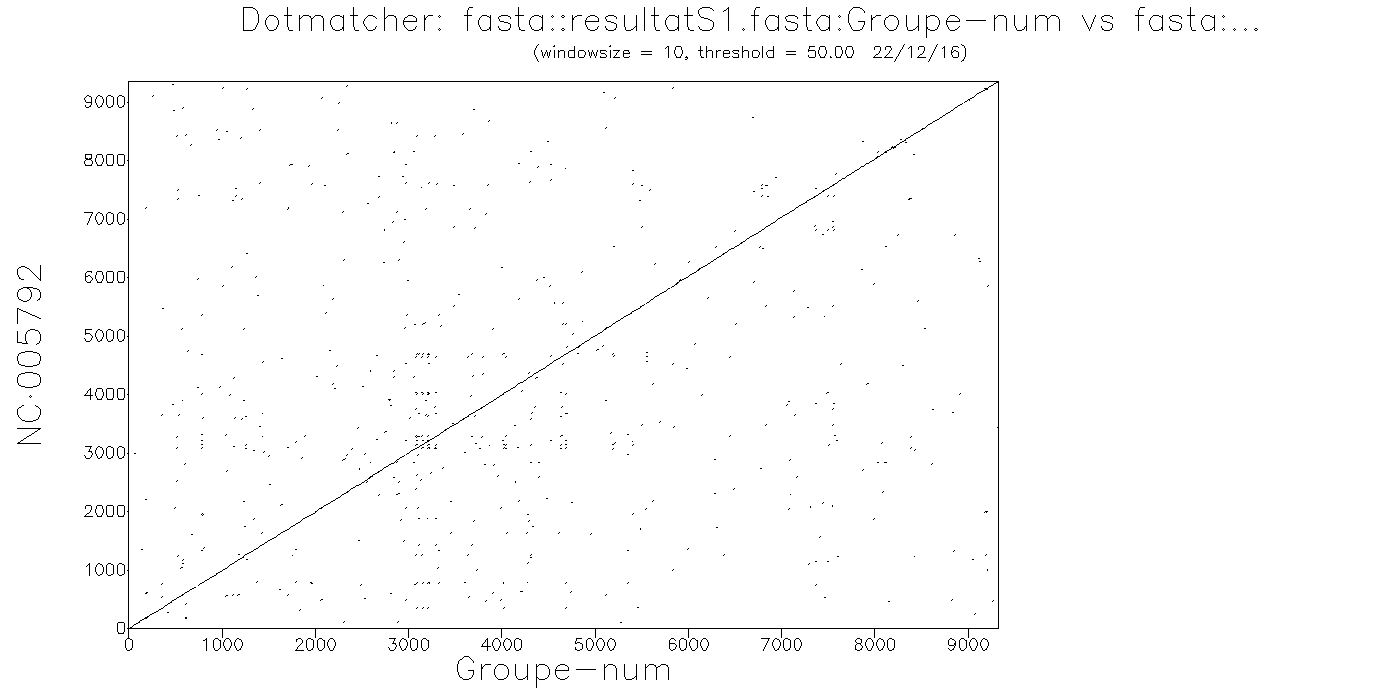
\includegraphics[scale=0.4]{dotmatcher1S.png}
\end{center}

Pour la collection 1, 4 et 5, nous voyons que les séquences cibles sont couvertes mais nos séquences sont trop grandes : environ le double à chaque fois.

\begin{center}
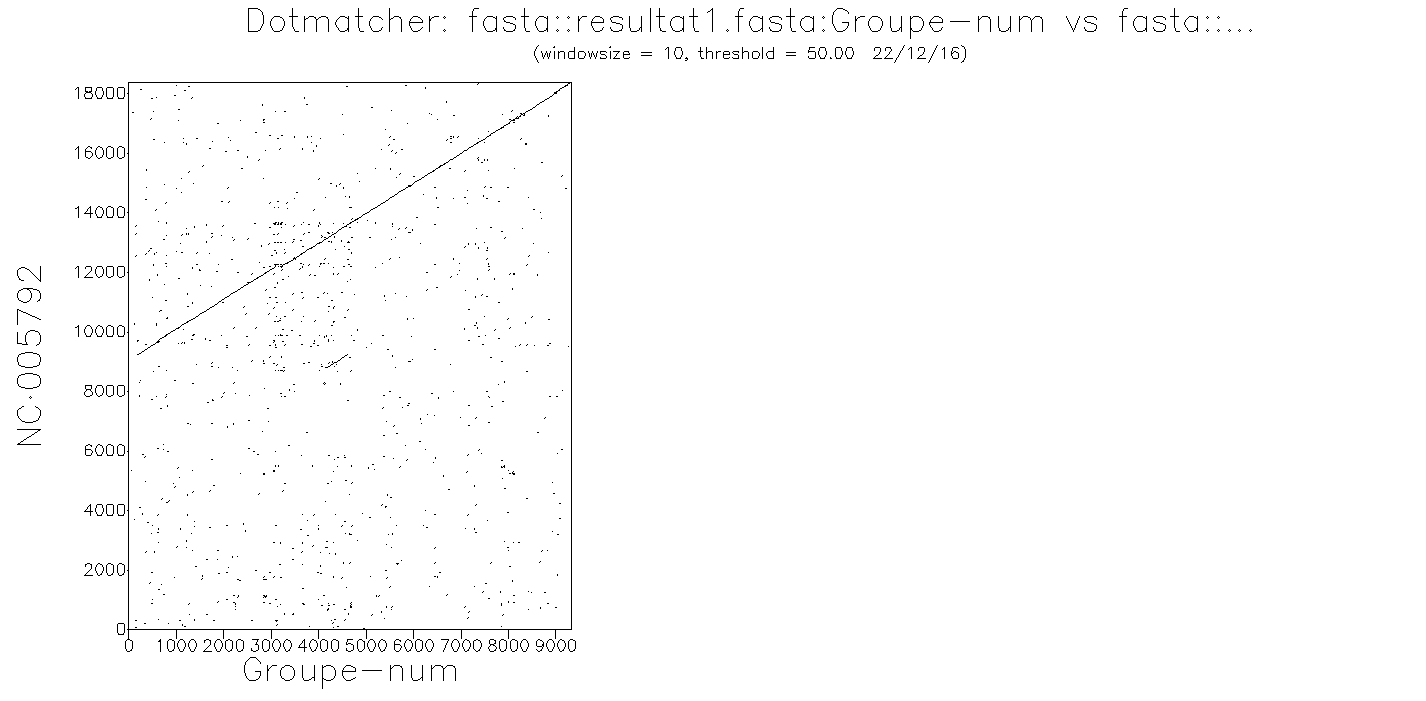
\includegraphics[scale=0.5]{dotmatcher1.png}
\end{center}

\begin{center}
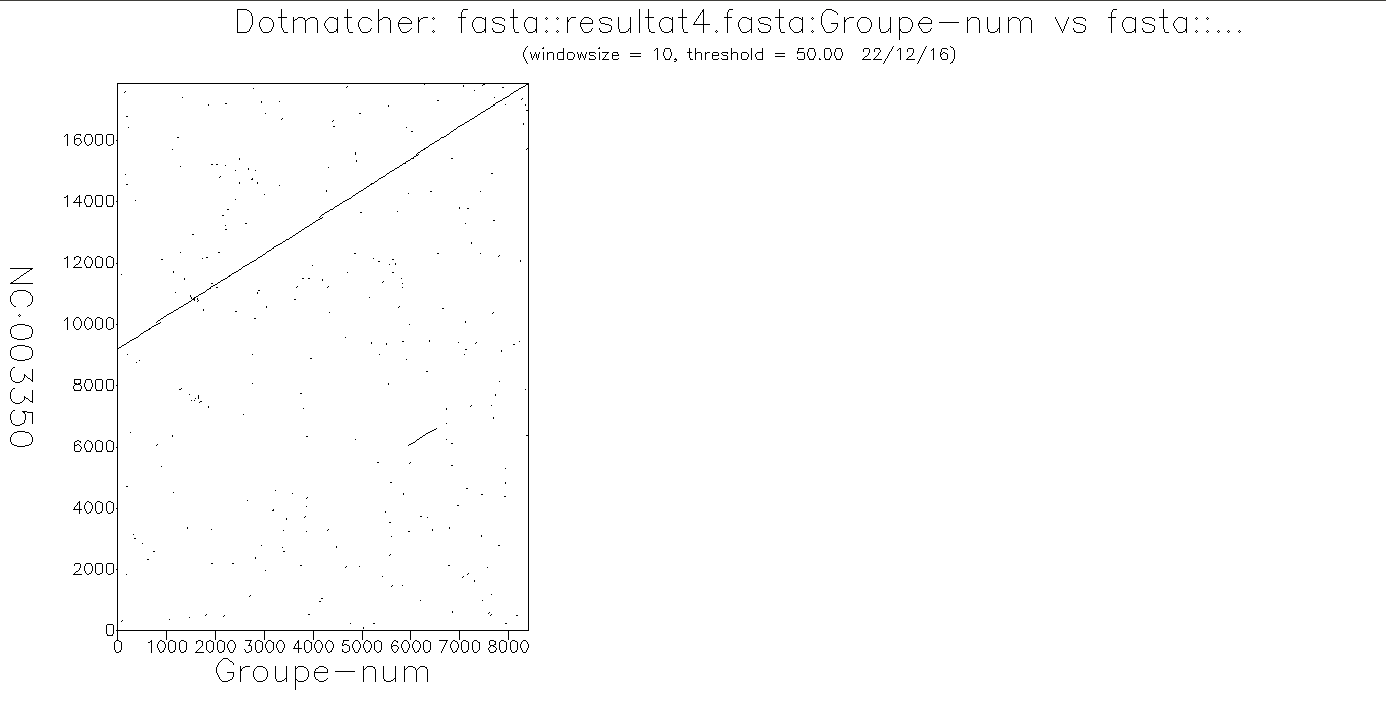
\includegraphics[scale=0.5]{dotmatcher4.png}
\end{center}

\begin{center}
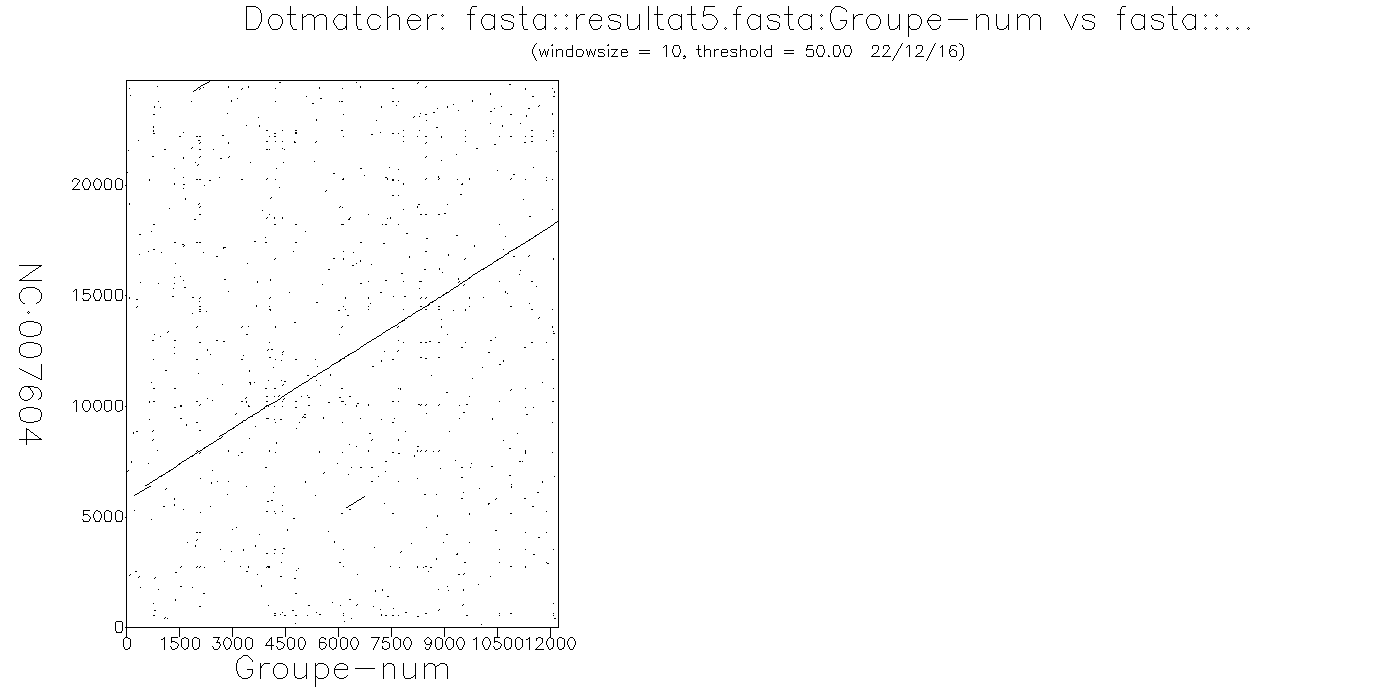
\includegraphics[scale=0.5]{dotmatcher5.png}
\end{center}

Le dotmatcher de la collection 2 est beaucoup plus floue. On peut voir que encore une fois toute la séquence est recouverte malgré qu'elle soit plus éparpillée. Sa taille est aussi trop grande.
\begin{center}
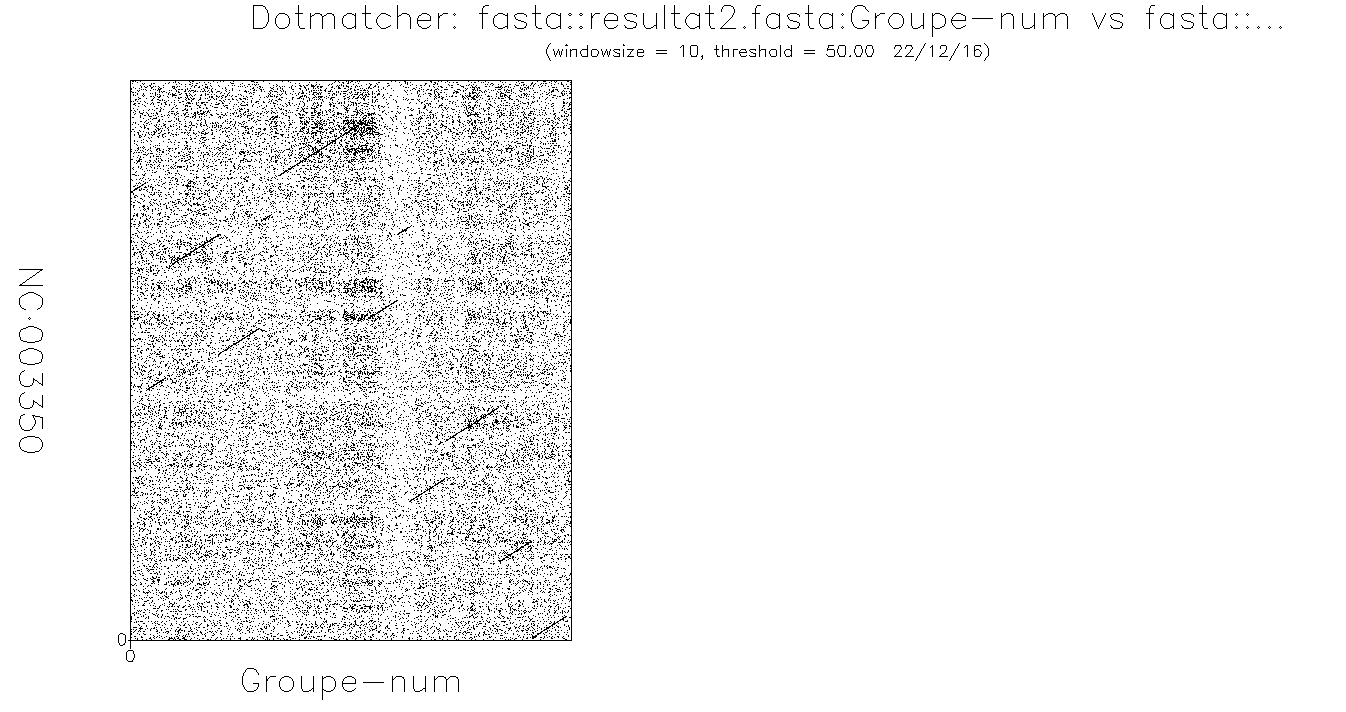
\includegraphics[scale=0.5]{dotmatcher2.png}
\end{center}

\newpage
\section{Conclusion}
L'assemblage de fragments est un problème très complexe. Il faut parvenir gérer une très grande quantité de données. De plus l'approximation de type Greedy exclu certaines possibilités d'assemblage : nous sommes obligés d'assembler les fragments en escalier. Or, en réalité, ils se chevauchent sûrement tous de manière aléatoire.  \\
\begin{center}
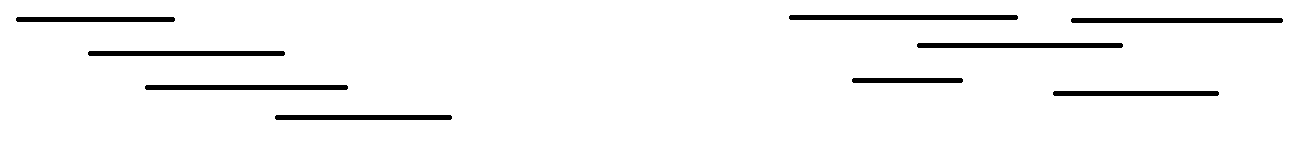
\includegraphics[scale=0.5]{alignement1.png}
\end{center}

Nous pensons que cela à un impact sur la longueur des séquences obtenues. \\

Nous avons eu des difficultés au niveau de la bonne compréhension des alignements afin d'effectuer le minimum de Semi-global et de stocker le minimum de liens. Comme nous stockons moitié moins de liens que ce qu'il existe en réalité, il a fallu retrouver quels alignements avaient les mêmes coûts et les remettre dans le bon sens. 
\end{document}
